\gdef\thisproblemauthor{}
\gdef\thisproblemdeveloper{}
\gdef\thisproblemorigin{}
\begin{problem}{飢餓的Sana}
{standard input}{standard output}
{1 seconds}{512 MB}{}

\centerline{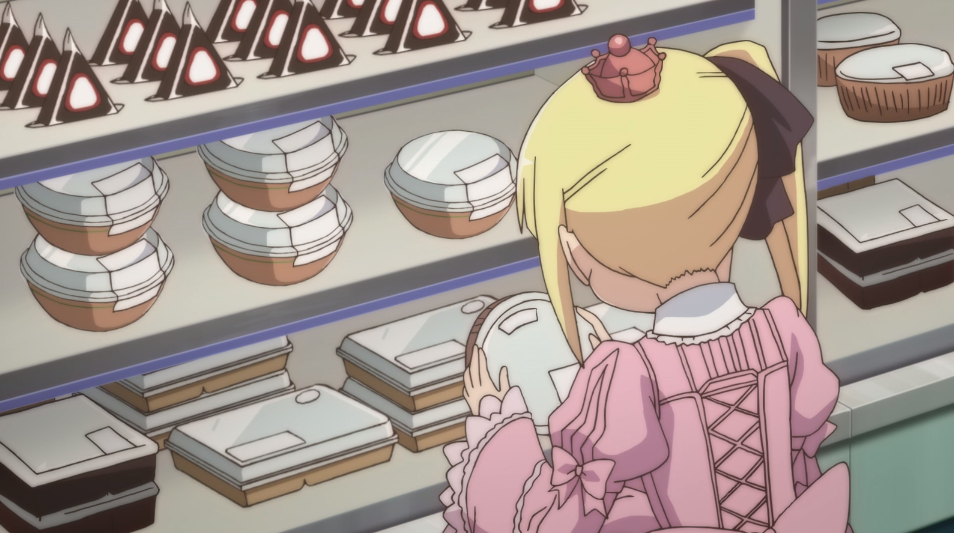
\includegraphics[scale=0.5]{./pics/B.png}}

$Sana$在使用大量能力之後會變的非常飢餓,因此她跑到了洞穴附近的一家超商想要大肆搜刮各種食物。在超商中有$K$個食物排列在一個直線的展示架上,由左而右數過去的第$i$個食物可以帶給Sana $w_i$的飽食度,若Sana吃了多樣食物,獲得的飽食度是所有吃下食物飽食度的總和。

飢餓的Sana會在超商中抓起連續一排的食物吃下去。因為Sana真的很餓,因此她至少會選一個食物吃掉,可是吃太多東西會讓她的肚子很不舒服,因此Sana想要選擇所有選取的可能中,飽食度第$K$大的選法,你知道聰明的Sana吃掉這些食物後,會獲得多少飽食度嗎?

\InputFile

只有一筆輸入。第一行有兩個數字$N~K$表示有$N$個食物,Sana會選擇第$K$大的選法。第二行有$N$個正整數,第$i$個數字$w_i$表示第$i$個食物的飽食度。

\begin{iofmt}
\begin{itemize}
	\item $1 \leq N \leq 10^5$
	\item $1 \leq K \leq min(\frac{N\times(N+1)}{2},10^9)$
	\item $1\leq w_i \leq 10^4$
\end{itemize}
\end{iofmt}

\OutputFile

請輸出食用完畢後,Sana獲得的飽食度為何。

\Examples

\begin{example}
\exmpfile{./sample/PB.sample.in}{./sample/PB.sample.out}%
\end{example}

\Examples
\begin{example}
\exmpfile{./sample/PB.sample2.in}{./sample/PB.sample2.out}%
\end{example}


\Explanations

在第二筆測資中,所有可能的選法有$(1,2,3),(2,3),(1,2),(3),(2),(1)$,故第四大的方法可以獲得$3$的飽食度。

\end{problem}
